
% ==========================================================
\section{Analytical Model}
\label{sec:analytical_model}

This section studies two implications of housing access in a two-period
overlapping-generations economy.  A financing-constrained young buyer can value
family-sized space more than an old incumbent.  We also compare two positive
steady states and compute a terminally closed adjustment after a permanent
change in desired fertility.  In the numerical construction, that adjustment
generates house-price appreciation and taxable gains even though gains vanish
at either endpoint.  Appendix~\ref{app:olg_proofs} gives the household
solutions, transition results, and mixed-tenure construction.

\subsection{Environment}

\textbf{Households.}
At date $t$, the economy contains $Y_t$ young households and $O_t$ old
households.  A young household has income $y_i$, liquid wealth $b_i$, and
chooses total nondurable expenditure $c$, total housing $h$, completed
fertility $n$, saving $a'$, and tenure $m\in\{R,O\}$.  The pair $(y_i,b_i)$ is
drawn from a fixed distribution $F$ in each cohort; estates are warm-glow
expenditures rather than the source of the next cohort's $b_i$.

\textbf{Preferences.}
Each child uses $\chi>0$ units of goods and $\kappa>0$ units of housing.  Define
the parts of the household bundle available to the adults as
\begin{equation}
 x=c-\chi n>0,\qquad s=h-\kappa n>0.
 \label{eq:olg_usable_bundles}
\end{equation}
Young and old flow utilities are
\begin{align}
 u_t^Y(c,h,n)&=\log(c-\chi n)+\alpha\log(h-\kappa n)
 +\vartheta_t\log n,
 \label{eq:olg_young_utility}\\
 u^2(c^2,h^2,e)&=\log c^2+\gamma\log h^2+\omega_B\log e.
 \label{eq:olg_old_utility}
\end{align}
Here $e$ is a warm-glow estate.  Writing both $c$ and $h$ as gross choices makes
the two child requirements parallel: both reduce the household bundle left for
the adults.  Logarithmic utility keeps conditional demands and the response to
a binding housing limit in closed form; the mechanisms themselves enter through
access constraints and tax timing.

\textbf{Demography.}
A child born at $t$ produces $\nu>0$ young households at $t+1$, after survival
and household formation.  Thus
$Y_{t+1}=\nu\bar n_tY_t$ and $O_{t+1}=Y_t$, where $\bar n_t$ is average
fertility among the young.

\textbf{Housing and asset markets.}
The fixed housing stock is $\bar H$.  Rental units satisfy
$h\leq h_R^{\max}$, owner units satisfy $h\leq h_O^{\max}$, and
$h_R^{\max}<h_O^{\max}$.  The consumption good is the numeraire, and the
economy can trade it through a one-period bond with price $q\in(0,1)$ and gross
return $R_f=q^{-1}$; only the housing market must clear domestically.  The
property tax applies to every housing unit and is paid by the owner of record.
Owner-occupiers pay it directly; for a rental unit, the landlord is a
competitive intermediary that can trade the bond.  The intermediary buys one
unit for $P_t$ at the beginning of date $t$.  At the end of the period it
collects rent $r_t$, pays property tax $\tau^pP_t$, and carries a unit worth
$P_{t+1}$.  Since $R_f=q^{-1}$ is the gross return between the beginning and end
of the period, free entry imposes
\begin{equation}
 r_t+P_{t+1}=R_fP_t+\tau^pP_t
 \quad\Longleftrightarrow\quad
 r_t=(R_f+\tau^p)P_t-P_{t+1}.
 \label{eq:olg_rental_user_cost}
\end{equation}
Thus $r_t$ is paid in date-$(t+1)$ goods and $q\,r_t$ is its date-$t$ value.
Household budgets are written in beginning-of-period goods, so rent and the
property tax appear at their discounted values.  At a steady state,
$r=(R_f-1+\tau^p)P$.  Capital-gains taxation enters through owner-occupied
housing.  Rental intermediaries are not taxed on resale in the baseline, so
the gains tax does not enter \eqref{eq:olg_rental_user_cost}.  Appendix
\ref{app:olg_reallocation} gives the corresponding incidence calculation when
intermediaries are also taxed.

\textbf{Capital-gains taxation and home finance.}
Household capital gains are taxed only upon sale.  An old owner who bought one
unit at $P_{t-1}$ and sells it at $P_t$ pays the tax per unit
\begin{equation}
 \ell_t=\tau^g\max\{P_t-P_{t-1},0\},
 \label{eq:olg_prices}
\end{equation}
where $\tau^g$ is the capital-gains tax rate.  The owner pays tax only when
$P_t>P_{t-1}$.  If the owner keeps the house until death, appreciation accrued
during the owner's life is not taxed.  The estate's tax basis is reset to the
date-$(t+1)$ price, so an immediate estate sale realizes no taxable gain.  The
estate sale returns the unit to the fixed stock, and its proceeds enter the
warm-glow estate and leave the economy.  Selling while alive therefore
triggers a tax that retaining the unit avoids.  A young buyer finances the share
$\phi\in(0,1)$ and therefore posts $(1-\phi)P_th$ at purchase.

\subsection{Household problems}

Households take prices and transfers as given.  A renter buys housing services
and carries only financial wealth into old age.  An owner buys housing, posts a
down payment before receiving current income, and carries both mortgage debt
and the house into old age.

\textbf{Young renters.}
Conditional on renting, the young household solves
\begin{align}
 W_t^R(i)=\max_{c,h,n,a'}\;&u_t^Y(c,h,n)+\beta V_{t+1}^R(R_fa') \\
 \text{s.t.}\quad&
 c+a'+q\,r_th=y_i+b_i+T_t,\nonumber\\[-2pt]
 &h\leq h_R^{\max},\qquad a'\geq0.
 \label{eq:olg_young_renter}
\end{align}
The renter pays for housing services each period and enters old age with
financial wealth $R_fa'$.

\textbf{Young owners.}
Conditional on owning, the young household solves
\begin{align}
 W_t^O(i)=\max_{c,h,n,a'}\;&u_t^Y(c,h,n)+\beta V_{t+1}^O(a_{t+1},h) \nonumber\\
 \text{s.t.}\quad&
 c+a'+[(1-\phi)+q\tau^p]P_th=y_i+b_i+T_t,\nonumber\\[-2pt]
 &a_{t+1}=R_fa'-R_f\phi P_th,\qquad
 (1-\phi)P_th\leq b_i,\qquad h\leq h_O^{\max},\qquad a'\geq0.
 \label{eq:olg_young_owner}
\end{align}
The closing occurs before current income and tax rebates are available, and
unsecured borrowing is unavailable.  Thus only beginning-of-period liquid
wealth $b_i$ can satisfy the down payment.  The transfer $T_t$ is the date-$t$
present value of the equal per-household rebate of housing-tax revenue.

\textbf{Old households.}
An old household has financial wealth $a$.  An owner also carries housing $H$
from young age.  Renters and owners solve, respectively,
\begin{align}
 V_t^R(a)&=\max_{c^2,h^2,e}u^2(c^2,h^2,e),
 &c^2+qe+q\,r_th^2&=a+T_t,\quad 0<h^2\leq h_R^{\max},
 \label{eq:olg_old_renter}\\
 V_t^O(a,H)&=\max_{c^2,h^2,e}u^2(c^2,h^2,e),
 &c^2+qe+(q\,r_t-\ell_t)h^2&=a+(P_t-\ell_t)H+T_t,\nonumber\\[-2pt]
 &&0<h^2&\leq H,\quad e\geq P_{t+1}h^2.
 \label{eq:olg_old_owner}
\end{align}
The marginal cost of retaining a unit is therefore $q\,r_t-\ell_t$: selling
realizes the current tax, while retaining the unit avoids it.

\textbf{Tenure choice.}
Each household draws once an idiosyncratic preference $\xi_i$ for ownership,
independently of $(y_i,b_i)$, and observes it before choosing tenure.  It owns
when $W_t^O(i)+\xi_i\geq W_t^R(i)$.  Assume $\xi_i$ is logistic with
location $\bar\xi$ and scale $\sigma_\xi>0$, which gives the owner share
\begin{equation}
 \pi_t^O(i)=
 \frac{\exp\{[W_t^O(i)+\bar\xi]/\sigma_\xi\}}
 {\exp\{W_t^R(i)/\sigma_\xi\}+\exp\{[W_t^O(i)+\bar\xi]/\sigma_\xi\}}.
\label{eq:olg_owner_share}
\end{equation}
This cross-sectional preference heterogeneity makes aggregate tenure shares
smooth.  It does not enter the conditional renter or owner policies.

\subsection{Housing constraints and the cost of children}

Desired housing is the amount a household would choose without the rental or
down-payment limit.  The access constraint binds when this amount exceeds the
housing the household can obtain.  Its shadow value measures willingness to
pay for one more unit.

Fix a household $i$, a date $t$, and a tenure choice $m\in\{R,O\}$.  To obtain
closed forms, first suppose that saving and the household's old-age choices are
interior.  Let
$A=1+\gamma+\omega_B$ denote the sum of the old-age expenditure weights, and
let lifetime resources, valued at date $t$, be
\begin{equation}
 w_{it}=y_i+b_i+T_t+qT_{t+1}.
 \label{eq:olg_lifetime_objects}
\end{equation}
The current cost of housing depends on tenure:
\begin{equation}
 u_t^R=q\,r_t,\qquad u_t^O=q(r_t+\ell_{t+1}).
 \label{eq:olg_tenure_user_costs}
\end{equation}
A renter pays the present value of rent.  A buyer faces the same opportunity
cost and, if the unit is sold in old age, the anticipated gains tax.  Solving
the saving and old-age choices reduces the lifetime problem, up to a constant,
to
\begin{align}
 \max_{x,s,n}\quad &(1+\beta A)\log x+\alpha\log s+
 \vartheta_t\log n \nonumber\\
 \text{s.t.}\quad &(1+\beta A)x+u_t^m s+
 (\chi+\kappa u_t^m)n=w_{it}.
 \label{eq:olg_interior_lifetime_problem}
\end{align}
The term $\beta A$ summarizes old-age demand for consumption, housing, and the
estate.  With logarithmic utility, these three uses receive fixed expenditure
shares, so the same term appears in the reduced objective and budget.  The last
term in the budget gives the full resource cost of another child: $\chi$ units
of goods and $\kappa$ units of housing valued at the tenure-specific user cost.

Without a housing-access constraint, define
$D_t=1+\beta A+\alpha+\vartheta_t$.  The household then chooses usable goods,
usable housing, and fertility according to
\begin{equation}
 x^m=\frac{w_{it}}{D_t},\qquad
 s^m=\frac{\alpha w_{it}}{D_tu_t^m},\qquad
 n^m=\frac{\vartheta_t w_{it}}
 {D_t(\chi+\kappa u_t^m)}.
 \label{eq:olg_interior_policies}
\end{equation}
Gross choices are $c^m=x^m+\chi n^m$ and $h^m=s^m+\kappa n^m$.

Access may prevent the household from choosing this amount of housing.  A
renter cannot exceed the largest rental unit, while a buyer cannot exceed
either the largest owner unit or the amount supported by liquid wealth:
\begin{equation}
 \widehat h_{it}^R=h_R^{\max},\qquad
 \widehat h_{it}^O=\min\left\{h_O^{\max},
 \frac{b_i}{(1-\phi)P_t}\right\}.
 \label{eq:olg_effective_caps}
\end{equation}
If desired gross housing in \eqref{eq:olg_interior_policies} is below this limit, the
constraint is irrelevant.  Otherwise the household sets $h^m=\widehat h_{it}^m$,
and usable consumption and fertility solve
\begin{align}
 (1+\beta A)x^m+\chi n^m+u_t^m\widehat h_{it}^m&=w_{it},
 \label{eq:olg_binding_budget}\\
 \frac{\vartheta_t}{n^m}
 &=\frac{\chi}{x^m}
 +\frac{\alpha\kappa}{\widehat h_{it}^m-\kappa n^m}.
 \label{eq:olg_binding_fertility_foc}
\end{align}
The second equation prices the goods and housing taken from the adult bundle by
another child.  The appendix proves that these two equations have a unique
interior solution on the stated branch.

The value of relaxing the housing limit is the household's marginal value of
space minus its user cost:
\begin{equation}
 \zeta_{it}^m=
 \frac{\alpha x^m}{s^m}-u_t^m\geq0.
 \label{eq:olg_access_wedge}
\end{equation}
It is zero when housing is unconstrained and positive when an access limit
binds with a positive multiplier.  If the owner's physical size limit is slack
and the down-payment constraint binds, denote this financial component by
$\zeta_{it}^{O,F}$.
Combining the housing and fertility conditions gives
\begin{equation}
 \frac{\vartheta_t x^m}{n^m}
 =\chi+\kappa\bigl(u_t^m+\zeta_{it}^m\bigr).
 \label{eq:olg_full_price_child}
\end{equation}
Thus a binding access constraint raises the effective cost of a child by
$\kappa\zeta_{it}^m$.  This is the direct link between housing access and
fertility.
When the rental limit also binds in old age, committed old-age rent changes the
lifetime budget.  Appendix~\ref{app:olg_young_households} gives that branch.

\subsection{Positive steady states and transitions}

A permanent change in desired fertility moves the economy between two steady
states.  House prices and taxable gains are constant at either endpoint, but
can change during the transition.

At an arbitrary date, let $\bar n_t$, $\bar h_t^Y$, and $\bar h_t^O$ denote
average fertility, young housing, and old housing generated by current choices
and the old-state distribution.  At constant prices, transfers, and
preferences, write their stationary counterparts as functions of $(P,T;
\vartheta)$, and let $\bar h(P,T;\vartheta)=\bar h^Y(P,T;\vartheta)+
\bar h^O(P,T;\vartheta)$.  Market clearing and the government budget are
\begin{align}
 Y_t\bar h_t^Y+O_t\bar h_t^O&=\bar H,
 \label{eq:olg_housing_clearing}\\
 (Y_t+O_t)T_t&=q\tau^pP_t\bar H+\ell_tO_t\bar h_t^{\mathrm{sell}},
 \label{eq:olg_government}
\end{align}
where $\bar h_t^{\mathrm{sell}}$ is housing sold by old owners per old household, assigning
zero sales to renters.

\begin{proposition}[Steady-state accounting]
\label{prop:olg_steady_state}
Every positive steady state satisfies
\begin{align}
 \bar n(P^*,T^*;\vartheta)&=\frac{1}{\nu},
 &\ell^*&=0,\\
 T^*&=\frac{q\tau^pP^*}{2}\bar h(P^*,T^*;\vartheta),
 &Y^*=O^*&=\frac{\bar H}{\bar h(P^*,T^*;\vartheta)}.
 \label{eq:olg_steady_state_system}
\end{align}
Stationarity fixes average fertility at the replacement rate.  Prices,
transfers, tenure, individual fertility and housing, and the population scale
can nevertheless differ across steady states.
\end{proposition}

Stationarity requires replacement fertility; household choices and housing
clearing determine the price and population scale consistent with it.  Appendix
\ref{app:olg_steady_states} gives conditions for local determination.

Suppose $\vartheta_t$ rises permanently at date zero.  The economy starts from
the old steady state, so $S_0=(Y^0,Y^0,G^0,P^0)$ and $P_{-1}=P^0$.  Because the
old at date $t$ made their choices when young at $t-1$, the state must keep
track of their financial wealth, housing, and tenure.  Let $G_t$ denote this
distribution and write $S_t=(Y_t,O_t,G_t,P_{t-1})$.  Given $S_0$, a transition
equilibrium is a sequence of prices, transfers, household
choices, tenure shares, and distributions such that households optimize, the
cohort and distribution laws hold, housing clears, the government budget
balances at every date, and the sequence converges to the new steady state.
The two market conditions are
\begin{align}
 Y_t\bar h_t^Y+O_t\bar h_t^O&=\bar H,\\
 (Y_t+O_t)T_t&=q\tau^pP_t\bar H+\ell_tO_t\bar h_t^{\mathrm{sell}}.
 \label{eq:olg_transition_residuals}
\end{align}
The first equation clears the housing market.  The second rebates property-tax
revenue and the gains taxes paid by old sellers.

Figure~\ref{fig:olg_mixed_transition} uses a finite terminal closure.  From date
$J+1$ onward, prices and transfers equal their new steady-state values.  The
last young cohort faces those values in old age, but its purchase price $P_J$
remains its tax basis, so $\ell_{J+1}$ can be nonzero.  Its induced state is
recorded rather than imposed.  The computed path satisfies equilibrium through
date $J$ and approximates the remaining infinite sequence.
Appendix~\ref{app:olg_transitions} states conditions for a locally determined
solution to each finite system and shows that extending the terminal date
barely changes the reported path.  These checks do not establish existence or
uniqueness of the infinite-horizon transition.

One permanent shock is sufficient for several cohorts to realize gains.  The
cohort law can be iterated as
\begin{equation}
 Y_t=Y_0\prod_{s=0}^{t-1}\nu\bar n_s,
 \qquad O_t=Y_{t-1}.
 \label{eq:olg_iterated_cohorts}
\end{equation}
The first fertility response therefore changes the next young cohort, which
later becomes old and produces another cohort.  With a fixed housing stock,
this sequence can move prices for more than two dates.  Whenever
$P_s>P_{s-1}$, the old cohort selling at $s$ realizes
$\ell_s=\tau^g(P_s-P_{s-1})>0$.  The preference change is the only exogenous
shock in the construction below; the sign and duration of appreciation are
properties of its computed equilibrium path.

\begin{figure}[!htb]
\centering
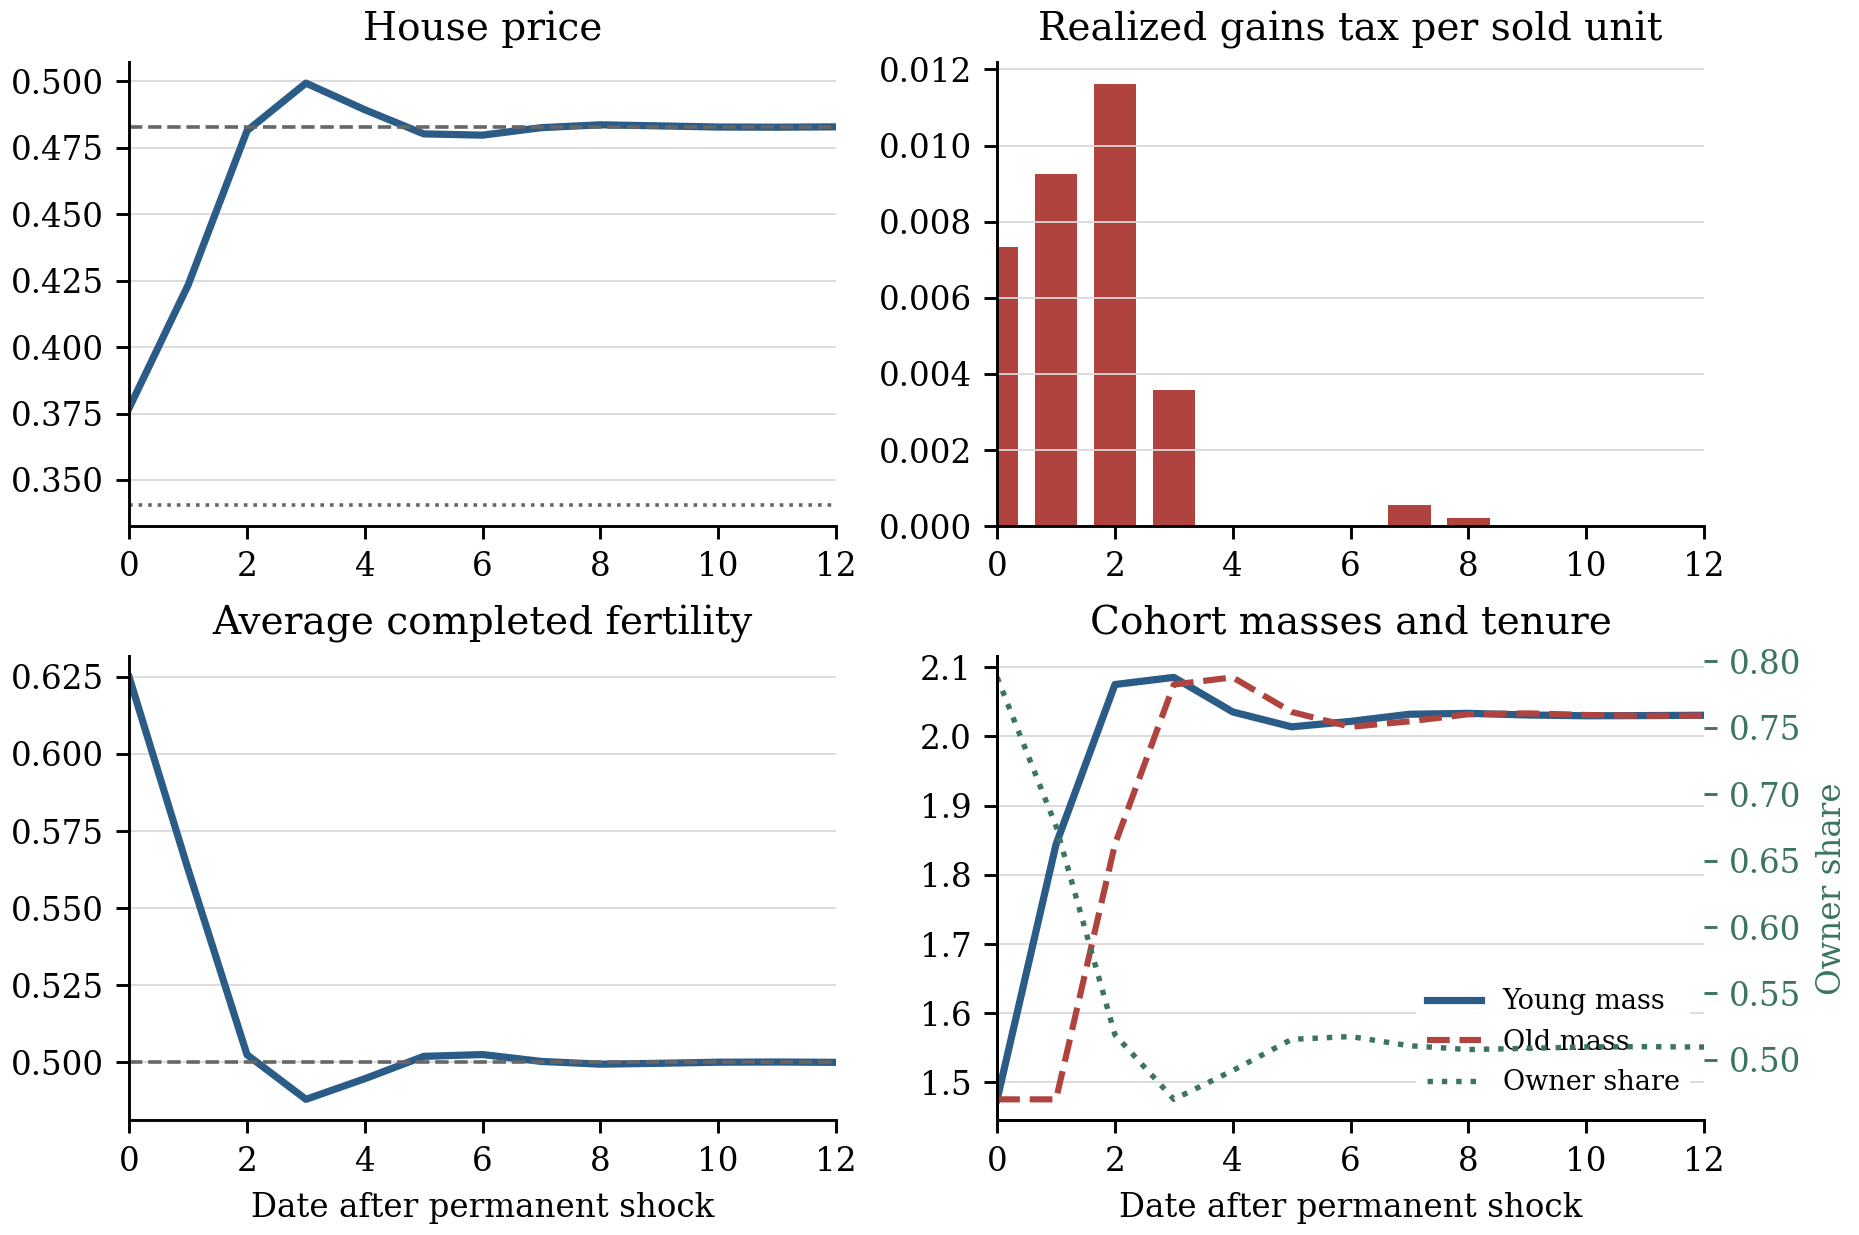
\includegraphics[width=0.55\textwidth]{figures/simplified_olg_mixed_tenure_transition.png}
\caption{Transition after a permanent increase in the fertility preference.
Lines mark steady-state prices and replacement fertility $1/\nu$.}
\label{fig:olg_mixed_transition}
\end{figure}

\subsection{Intergenerational reallocation and fertility}

Consider a marginal transfer of housing from an old incumbent to a young
owner, holding fertility, cohort sizes, tenure, prices, and other allocations
fixed.  The buyer's down-payment constraint binds; the other relevant choices
are interior.  Their marginal values of current housing services are
\begin{equation}
 MV_{it}^Y=q\,r_t+q\ell_{t+1}+\zeta_{it}^{O,F},
 \qquad
 MV_{jt}^O=q\,r_t-\ell_t.
 \label{eq:olg_marginal_values}
\end{equation}

The common term $q r_t$ is the value of housing services.  A sale costs the
incumbent $\ell_t$, the buyer anticipates $q\ell_{t+1}$, and the financing
constraint contributes $\zeta_{it}^{O,F}$.

Holding fertility, cohort sizes, and tenure fixed, call an allocation
\emph{conditionally locally efficient} if no small housing reallocation and
budget-balanced transfers can make all households alive at $t$ weakly better
off and one strictly better off.  Appendix~\ref{app:olg_reallocation} gives the
transfer scheme.

\begin{proposition}[Intergenerational reallocation]
\label{prop:olg_reallocation}
Under the conditions above and the two-date transfer ledger stated in
Appendix~\ref{app:olg_reallocation}, the marginal-value difference is
\begin{equation}
 MV_{it}^Y-MV_{jt}^O
 =\zeta_{it}^{O,F}+\ell_t+q\ell_{t+1}.
 \label{eq:olg_reallocation_surplus}
\end{equation}
Let $K_{ijt}\geq0$ be the marginal resource cost of transferring title and
occupancy.  Purchase and tax payments are transfers.  If
$MV_{it}^Y-MV_{jt}^O>K_{ijt}$, the allocation is not conditionally locally
efficient.
\end{proposition}

At a steady state the condition is $\zeta_i^{O,F}>K_{ij}$; the gains-tax terms
are transition-specific.  Thus the transfer improves the welfare of households
alive at $t$ when the value gap covers its resource cost.  The result does not
rank economies with different populations.

Let $\widehat h$ denote a binding housing limit.  Holding tenure, prices,
lifetime wealth, and the active set fixed, the interior old-age branch gives
\begin{equation}
 \frac{\dd n}{\dd\widehat h}\geq0
 \quad\Longleftrightarrow\quad
 \chi\leq
 \frac{(1+\beta A)\kappa(u_t^m+\zeta_{it}^m)^2}{\alpha u_t^m}.
\label{eq:olg_fertility_sign}
\end{equation}
Appendix~\ref{app:olg_fertility} derives this expression and the corresponding
capped-renter formula.
More accessible space raises fertility when children are sufficiently
space-intensive relative to their goods cost.  The same calculation gives
$\partial n/\partial w>0$ and $\partial n/\partial u_t^m<0$.  This is a
partial-equilibrium result; a funded policy also moves prices and transfers.
